% DPF 09 talk on strangeness in nucleon

\documentclass[10pt]{beamer}
\usepackage{amsmath}
\usefonttheme{professionalfonts} % using non standard fonts for beamer
\usefonttheme{serif} % default family is serif\
\usepackage{mathtools}
%\documentclass[12pt]{beamerthemeSam.sty}
\usepackage{epsf}
\usepackage{ulem}
\usepackage{array}
%\usepackage{pstricks}
%\usepackage[orientation=portrait,size=A4]{beamerposter}
\geometry{paperwidth=160mm,paperheight=120mm}
%DT favorite definitions
\def\LL{\left\langle}	% left angle bracket
\def\RR{\right\rangle}	% right angle bracket
\def\LP{\left(}		% left parenthesis
\def\RP{\right)}	% right parenthesis
\def\LB{\left\{}	% left curly bracket
\def\RB{\right\}}	% right curly bracket
\def\PAR#1#2{ {{\partial #1}\over{\partial #2}} }
\def\PARTWO#1#2{ {{\partial^2 #1}\over{\partial #2}^2} }
\def\PARTWOMIX#1#2#3{ {{\partial^2 #1}\over{\partial #2 \partial #3}} }

\def\rightpartial{{\overrightarrow\partial}}
\def\leftpartial{{\overleftarrow\partial}}
\def\diffpartial{\buildrel\leftrightarrow\over\partial}

\def\BI{\begin{itemize}}
\def\EI{\end{itemize}}
\def\BE{\begin{displaymath}}
\def\EE{\end{displaymath}}
\def\BEA{\begin{eqnarray*}}
\def\EEA{\end{eqnarray*}}
\def\BNEA{\begin{eqnarray}}
\def\ENEA{\end{eqnarray}}
\def\EL{\nonumber\\}
\def\BS{\bigskip}
\def\BC{\begin{center}}
\def\EC{\end{center}}
\def\BCC{\begin{columns}}
\def\ECC{\end{columns}}
\def\HC{\column{0.5\textwidth}}
\newcommand{\map}[1]{\frame{\frametitle{\textbf{Course map}}
\centerline{\includegraphics[height=0.86\paperheight]{../../map/#1.png}}}}
\newcommand{\wmap}[1]{\frame{\frametitle{\textbf{Course map}}
\centerline{\includegraphics[width=0.96\paperwidth]{../../map/#1.png}}}}

\newcommand{\etal}{{\it et al.}}
\newcommand{\gbeta}{6/g^2}
\newcommand{\la}[1]{\label{#1}}
\newcommand{\ie}{{\em i.e.\ }}
\newcommand{\eg}{{\em e.\,g.\ }}
\newcommand{\cf}{cf.\ }
\newcommand{\etc}{etc.\ }
\newcommand{\atantwo}{{\rm atan2}}
\newcommand{\Tr}{{\rm Tr}}
\newcommand{\dt}{\Delta t}
\newcommand{\op}{{\cal O}}
\newcommand{\msbar}{{\overline{\rm MS}}}
\def\chpt{\raise0.4ex\hbox{$\chi$}PT}
\def\schpt{S\raise0.4ex\hbox{$\chi$}PT}
\def\MeV{{\rm Me\!V}}
\def\GeV{{\rm Ge\!V}}

%AB: my color definitions
%\definecolor{mygarnet}{rgb}{0.445,0.184,0.215}
%\definecolor{mygold}{rgb}{0.848,0.848,0.098}
%\definecolor{myg2g}{rgb}{0.647,0.316,0.157}

\definecolor{A}{rgb}{0.8,0.0,0.0}
\definecolor{B}{rgb}{0.0,0.6,0.0}
\definecolor{C}{rgb}{0.4,0.4,0.0}
\definecolor{D}{rgb}{0.0,0.0,0.5}
\definecolor{E}{rgb}{0.4,0.4,0.4}


\definecolor{abtitlecolor}{rgb}{0.0,0.255,0.494}
\definecolor{absecondarycolor}{rgb}{0.0,0.416,0.804}
\definecolor{abprimarycolor}{rgb}{1.0,0.686,0.0}
\definecolor{Red}           {cmyk}{0,1,1,0}
\definecolor{Grey}           {cmyk}{.7,.7,.7,0}
\definecolor{Lg}           {cmyk}{.4,.4,.4,0}
\definecolor{Blue}          {cmyk}{1,1,0,0}
\definecolor{Green}         {cmyk}{1,0,1,0}
\definecolor{Brown}         {cmyk}{0,0.81,1,0.60}
\definecolor{Black}         {cmyk}{0,0,0,1}

\usetheme{Madrid}


%AB: redefinition of beamer colors
%\setbeamercolor{palette tertiary}{fg=white,bg=mygarnet}
%\setbeamercolor{palette secondary}{fg=white,bg=myg2g}
%\setbeamercolor{palette primary}{fg=black,bg=mygold}
\setbeamercolor{title}{fg=abtitlecolor}
\setbeamercolor{frametitle}{fg=abtitlecolor}
\setbeamercolor{palette tertiary}{fg=white,bg=abtitlecolor}
\setbeamercolor{palette secondary}{fg=white,bg=absecondarycolor}
\setbeamercolor{palette primary}{fg=black,bg=abprimarycolor}
\setbeamercolor{structure}{fg=abtitlecolor}

\setbeamerfont{section in toc}{series=\bfseries}

%AB: remove navigation icons
\beamertemplatenavigationsymbolsempty
\title{
  \textbf {More examples; angular momentum}\\
%\centerline{}
%\centering
%\vspace{-0.0in}
%\includegraphics[width=0.3\textwidth]{propvalues_0093.pdf}
%\vspace{-0.3in}\\
%\label{intrograph}
}

\author[W. Freeman] {Physics 211\\Syracuse University, Physics 211 Spring 2022\\Walter Freeman}

\date{\today}

\begin{document}

\frame{\titlepage}

\frame{\frametitle{\textbf{Announcements}}
	\large
\BI
\item{HW9 is due next Wednesday (last recitation of the semester)}
\item Help hours this week:
\item  Tuesday, 9:45-10:45ish (between classes)
\item Thursday, 9:45-10:45ish (between classes) and 1:30-3:30
\item Friday, 1:00-3:00
\BS\BS\pause
\item Have a study group of four or more? Let me know time and place and I will try to get you a tutor.
\BS\BS\pause
\item See the email announcement for more on makeups etc.\pause
\item {\bf Also in the email: what will be on the final}
\EI
}

\frame{\frametitle{\textbf{Final exam review}}
	\large
	
	I will rapidly get more free time once class is over.
	
	\BS\BS
	
	I am planning on holding 3-4 all-day review sessions between the last day of class and our final. 
	
	\BS\BS
	
	In the past, these have been smaller affairs with attendance 10-30.
	
	\BS\BS
	
	The idea of having so much time available is to spread students out, so that you can get personal help with your questions.
	
	\BS\BS
	
	I am working on scheduling these and will let you know when I have rooms locked in.
}


\frame{\frametitle{\textbf{Last time: combining translation and rotation}}
	\Large
	How do we analyze situations where objects both rotate and translate?
	
	\BS\BS
	
	\large
	
	\BI
\item 1. Draw force diagrams for all objects
\BI
\item Objects that rotate need extended force diagrams showing {\it where} forces act
\EI

\BS

\item {\color{Red}2. Write down {$\tau = I \alpha$} for all objects that might rotate}
\item {\color{Blue}3. Write down {$\vec F = m \vec a$} for all objects that might translate}
\BI
\item {\color{Blue}Sometimes the same object will do both}
\EI
\BS

\item 4. Apply the ``no-slip'' constraint if appropriate: $a = \pm \alpha r$ (think about which $r$)
\BI
\item Think carefully about direction: do $a$ and $\alpha$ have the same sign?
\EI

\BS

\item 5. Solve the system of equations
\BI
\item Often many of the $r$'s will cancel; sometimes they won't
\EI
\EI
}
		
		
		\frame{\frametitle{\textbf{An example}}
			
			\Large
			
			Which way does the spool move when I pull the ribbon to the side? What about straight up?
			
		}
	
	
	\frame{\frametitle{\textbf{Another example (8:00 only)}}
		
		\Large
		Which will make the weight fall faster?
		
		\BI
		\item A: Moving the masses inward
		\item B: Moving the masses outward
		\item C: Switching to a pulley with a larger radius
		\item D: Switching to a pulley with a smaller radius
		\EI
		
		\BS
		How fast does the weight accelerate downward?
	}
			
	
	\frame{\frametitle{\textbf{Another example (11:00 only)}}
		\Large
		
		Suppose a Ping-Pong ball is resting on a picnic table; the coefficient of static friction between them is $\mu_s$ and the Ping-Pong ball has a mass $m$. A gust of wind blows the ball, exerting a force $F_w$ to one side.
		
		\BS
		
		How large can the wind force be for the ball to still roll without slipping?
		
		
	}
	


\frame{\frametitle{\textbf{Angular momentum}}
	\begin{columns}
		\column{0.5\textwidth}
		\color{Grey}
		\Large
		\centerline{Translational motion}
		\normalsize
		\BI
		{\color{Red}
			\item{Moving objects have momentum}
			\item{$\vec p = m \vec v$}
			\item{Momentum conserved if there are no external forces}}
		\EI
		\column{0.5\textwidth}
		\color{Grey}
		\Large
		\centerline{Rotational motion}
		\normalsize
		\BI
		{\color{Blue}
			\item{Spinning objects have angular momentum $L$}
			\item{$L = I \omega$}
			\item{Angular momentum conserved if no external torques}}
		\EI
	\end{columns}
	
	\bigskip
	\bigskip
	
	\Large
	\color{Red}
	
	$\rightarrow$ $L = I \omega = $ constant; analogue to conservation of momentum
	
}

\frame{\frametitle{\textbf{Conservation of angular momentum}}
	\large
	We saw that the conservation of momentum was valuable mostly in two sorts of situations:
	
	\BI
	\item{Collisions: two objects strike each other}
	\item{Explosions: one object separates into two}
	\EI
	
	There is a third common case for conservation of angular momentum:
	
	\BI
	\item{Collisions: a child runs and jumps on a merry-go-round}
	\item{Explosions: throwing a ball off-center}
	\item{{\color{Red}A spinning object changes its moment of inertia}}
	\EI
	
	\pause
	\bigskip
	
	This last happens because moment of inertia depends on {\it how the mass is distributed}, not just how much there is!
}

\frame{\frametitle{\textbf{Conservation of angular momentum}}
	
	\Large
	\BC
	
	These problems are approached in exactly the same way as conservation of 
	{\it linear} momentum problems: write down expressions for $L_i$ and $L_f$ 
	and set them equal (if there are no external torques).
	
	\Huge
	
	$$L = I \omega$$
	
	$$\sum L_i=\sum L_f$$ \\
	
	\EC
}


\frame{
	
	\Large
	
	What will happen when I pull the string, collapsing the ball?

\BI
\item A: The ball will rotate faster
\item B: The ball will rotate slower
\item C: Nothing will happen \pause
\item The bolt connecting the ball to the ceiling will fail, and the whole thing will fall on my head
\EI
}



\frame{\frametitle{\textbf{Conservation of angular momentum}}
	\Large
	If I kept the mass of the Earth the same, but enlarged it so that it had twice
	the diameter, how long would a day be?
	
	\BS
	
	(Remember, the total angular momentum, $L=I\omega$, stays the same)
	
	\BS
	\BS
	
	\Huge
	
	\color{A}A: 6 hours\\
	\color{B}B: 12 hours\\
	\color{C}C: 24 hours\\
	\color{D}D: 48 hours\\
	\color{E}E: 96 hours\\
}



\frame{
	
	\Large
	
	What will happen the person on the platform turns the wheel over?
	
	\BI
	\item A: Nothing will happen
	\item B: They will rotate counterclockwise
	\item C: They will rotate clockwise
	\item D: They will stop rotating
	\EI
}



\frame{\frametitle{\textbf{Angular momentum of a single object}}

\large

A single object moving in a straight line also has angular momentum.
\Huge
$$L = mv_\perp r = mvr_\perp$$
\large

\BS
\BS
\BS

\BCC
\HC
If we are to trust this relation, then the angular momentum of an object moving 
with constant $\vec v$ should be constant!

\BS

Is the angular momentum the same at points A and B?
\HC
\BC
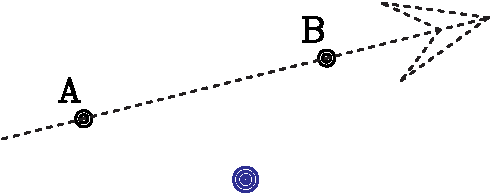
\includegraphics[width=0.8\textwidth]{angmombare-crop.pdf}
\EC
\ECC
}


\frame{\frametitle{\textbf{Angular momentum of a single object}}

\large

A single object moving in a straight line also has angular momentum.
\Huge
$$L = \color{Lg}mv_\perp r =\color{Red} mvr_\perp$$
\large

\BS
\BS
\BS

\BCC
\HC
Is the angular momentum the same at points A and B?

\BS

\color{Red}
Yes: $r_\perp$ (and $v$) are the same at both points.

\HC
\BC
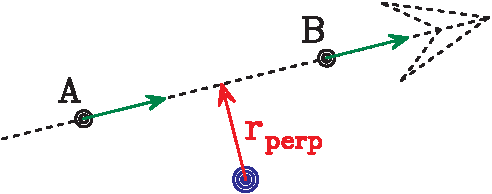
\includegraphics[width=0.8\textwidth]{angmom-crop.pdf}
\EC
\ECC
}

%\frame{\frametitle{\textbf{An example problem}}
%\Large
%A child of mass $m$ runs at speed $v$ straight east and jumps onto a merry-go-round of mass $M$ and radius $R$,
%landing $2/3$ of the way toward the outside. If she lands on the south edge,
%how fast will it be turning once she lands?
%
%\BS
%
%We'll do this together on the document camera.
%
%\pause
%
%\BS\BS
%\BC\it\normalsize
%
%(The solution is on the next slide, for those studying these notes later)
%\EC
%}
%
%\frame{\frametitle{\textbf{The solution to our example}}
%\large
%
%We use conservation of angular momentum:
%
%\begin{align*}
%\sum L_i &= \sum L_f \\
%L_{\rm child,\it i}  &= L_{\rm child+disk,\it f}
%\end{align*}
%
%Model the child as a point object moving at a constant velocity:
%$$L_{\rm child,\it i} = mv_\perp r = \frac{2}{3} mvR$$
%
%This gives us $\frac{2}{3}mvR = I_{\rm total} \omega_f$. We now need $I_{\rm total}$.
%
%\medskip
%
%After the child jumps on, $I_{\rm total} = I_{\rm disk} + I_{\rm child} = \frac{1}{2}MR^2 + \frac{2}{3}mR^2$. Thus,
%
%$$\frac{2}{3}mvR = \left(\frac{1}{2}MR^2 + \frac{2}{3}mR^2\right) \omega_f$$
%
%Solve for $\omega_f$:
%
%$$
%\omega_f = \frac{\frac{2}{3}mvR}{\left(\frac{1}{2}MR^2 + \frac{2}{3}mR^2\right)}
%$$
%
%}


\frame{\frametitle{\textbf{Angular momentum demonstrations}}

\Large

What happens to the person on the platform if they catch the ball?

\pause

What happens when they throw it?
}






%
%\frame{\frametitle{\textbf{Review: The work-energy theorem}}
%
%\Large
%\BI
%
%\item Translational work-energy theorem: $\frac{1}{2}mv_f^2 - \frac{1}{2}mv_i^2 = \vec F \cdot \vec d = F d \cos \theta$ (if this is constant)
%
%\item Rotational work-energy theorem: $\frac{1}{2}I\omega_f^2 - \frac{1}{2}I\omega_i^2 = \tau \Delta \theta$
%
%\EI
%
%
%\BS\BS
%
%Potential energy is an alternate way of keeping track of the work done by conservative forces:
%
%\BI
%\item $PE_{\rm grav} = mgh$
%\item $PE_{\rm spring} = \frac{1}{2}kx^2$
%\EI
%
%
%
%}
%
%
%\frame{\frametitle{\textbf{Review: Conservation of energy}}
%
%\BC
%\begin{tabular}{ccccccccc}
%\large $\color{Blue}{\large \rm PE_i} $
%&\large+&\large$\color{Red} \frac{1}{2}mv_i^2 + \frac{1}{2}I\omega_i^2$
%&\large+&\large$ W_{\rm other} $
%&\large=&\large$\color{Blue}{\rm PE_f} $
%&\large+&\large$\color{Red} \frac{1}{2}mv_f^2 + \frac{1}{2}I\omega_f^2$ \\
%\pause
%\\
%\color{Blue}(initial PE) &+& \color{Red} (initial KE) &+& (other work) &=&\color{Blue} (final PE) &+&\color{Red}(final KE) \\
%\pause
%\\
%\multicolumn{3}{c}{(total initial mechanical energy)}  &+& (other work) &=& \multicolumn{3}{c}{(total final mechanical energy)} \\
%%&+& (other work) &=& \multicolumn{3}{c}{(total final mechanical energy)}\\
%\end{tabular}
%
%\BS
%\BS
%\pause
%
%\Large Since conservation of energy is the broadest principle in science, it's no surprise that we can do this!
%
%\EC
%}
%
%\frame{\frametitle{\textbf{Review: rotational motion}}
%
%\begin{center}
%\begin{tabular}{l | l}
%
% \multicolumn{1}{c|}{\Large Translation} & \multicolumn{1}{c}{\Large Rotation} \\
% \\
%\hline
%\hline
% & \\
%Position $\vec s$ & Angle $\theta$ \\
%Velocity $\vec v$ & Angular velocity $\omega$ \\
%Acceleration $\vec a$ & Angular acceleration $\alpha$ \\
% & \\
%\hline
%\hline
% & \\
%Kinematics: $\vec s(t)\frac{1}{2}\vec at^2 + \vec v_0 t + \vec s_0$ & $\theta(t) = \frac{1}{2}\alpha t^2 + \omega_0 t + \theta_0$ \\
% & \\
%\hline
%\hline
%
% & \\
%Force $\vec F$ & Torque $\tau$ \\
%Mass $m$ & Rotational inertia $I$ \\
%Newton's second law $\vec F = m \vec a$ & Newton's second law for rotation $\tau = I \alpha$ \\
% & \\
%
%\hline
%\hline
%
% & \\
%Kinetic energy $KE=\frac{1}{2}mv^2$ & Kinetic energy $KE=\frac{1}{2}I\omega^2$ \\
%Work $W = \vec F \cdot \Delta \vec s$ & Work $W = \tau \Delta \theta$ \\
%Power $P = \vec F \cdot \vec v$ & Power $P = \tau \omega$ \\
% & \\
%
%\hline
%\hline
%
% & \\
%Momentum $\vec p = m \vec v$ & Angular momentum $L = I\omega$\\
% & \\
%
%\hline
%\end{tabular}
%\end{center}
%}
%
%\frame{\frametitle{\textbf{Review: computing torques and static equilbrium}}
%
%\Large
%
%``Signpost problem'' from recitation
%}
%
%\frame{\frametitle{\textbf{Review: combining translational and rotational motion}}
%
%\Large
%
%``Yo-yo problem'' from recitation}
%
%\frame{
%
%\Huge
%\BC
%What would you like to talk about?
%\EC
%}

\end{document}

